\section{Einleitung}

Durch Stechmücken übertragene Krankheiten stellen in vielen tropischen und subtropischen Regionen weiterhin ein erhebliches Gesundheitsproblem dar. Eine besondere Rolle spielt dabei die Mücke \textit{Aedes aegypti}, die unter anderem als Überträger von Dengue-, Zika- und Chikungunya-Viren bekannt ist. Da sich \textit{Aedes aegypti} besonders gut an urbane Umgebungen anpasst, entstehen potenzielle Brutstätten häufig in der unmittelbaren Nähe menschlicher Siedlungen. Dazu gehören beispielsweise Wassertanks, Eimer, Reifen, Abflüsse, Müllbehälter oder andere künstliche Objekte, in denen sich Wasser sammeln kann.

Eine gezielte Kontrolle solcher Brutstätten ist ein wichtiger Bestandteil der Vektorbekämpfung. In der Praxis ist die Identifikation potenzieller Brutstätten jedoch aufwendig, da große urbane Flächen regelmäßig untersucht werden müssen. Klassische Inspektionsverfahren erfordern viel Personal, Zeit und lokale Expertise. Gerade in dicht bebauten Gebieten ist es schwierig, alle relevanten Bereiche vollständig und effizient zu erfassen. Aus diesem Grund gewinnen bildbasierte Verfahren zunehmend an Bedeutung. Insbesondere unbemannte Luftfahrzeuge, sogenannte UAVs oder Drohnen, ermöglichen die Aufnahme hochauflösender Luftbilder und Videodaten urbaner Gebiete.

In Verbindung mit Verfahren des maschinellen Lernens können UAV-Daten genutzt werden, um potenzielle Brutstätten automatisch zu erkennen. Objekterkennungsmodelle wie YOLO sind in der Lage, relevante Objektklassen in Bildern zu lokalisieren und mit Bounding Boxes zu markieren. Dadurch entsteht die Möglichkeit, große Bild- oder Videodatenmengen schneller auszuwerten und menschliche Expertinnen und Experten bei der Inspektion zu unterstützen. Gleichzeitig stellt die automatische Erkennung kleiner Objekte in UAV-Aufnahmen eine besondere Herausforderung dar. Viele potenzielle Brutstätten sind im Bild nur wenige Pixel groß, teilweise verdeckt oder visuell schwer von komplexen Hintergrundstrukturen wie Dächern, Schatten, Straßenflächen oder technischen Installationen zu unterscheiden.

\begin{figure}[htbp]
    \centering
    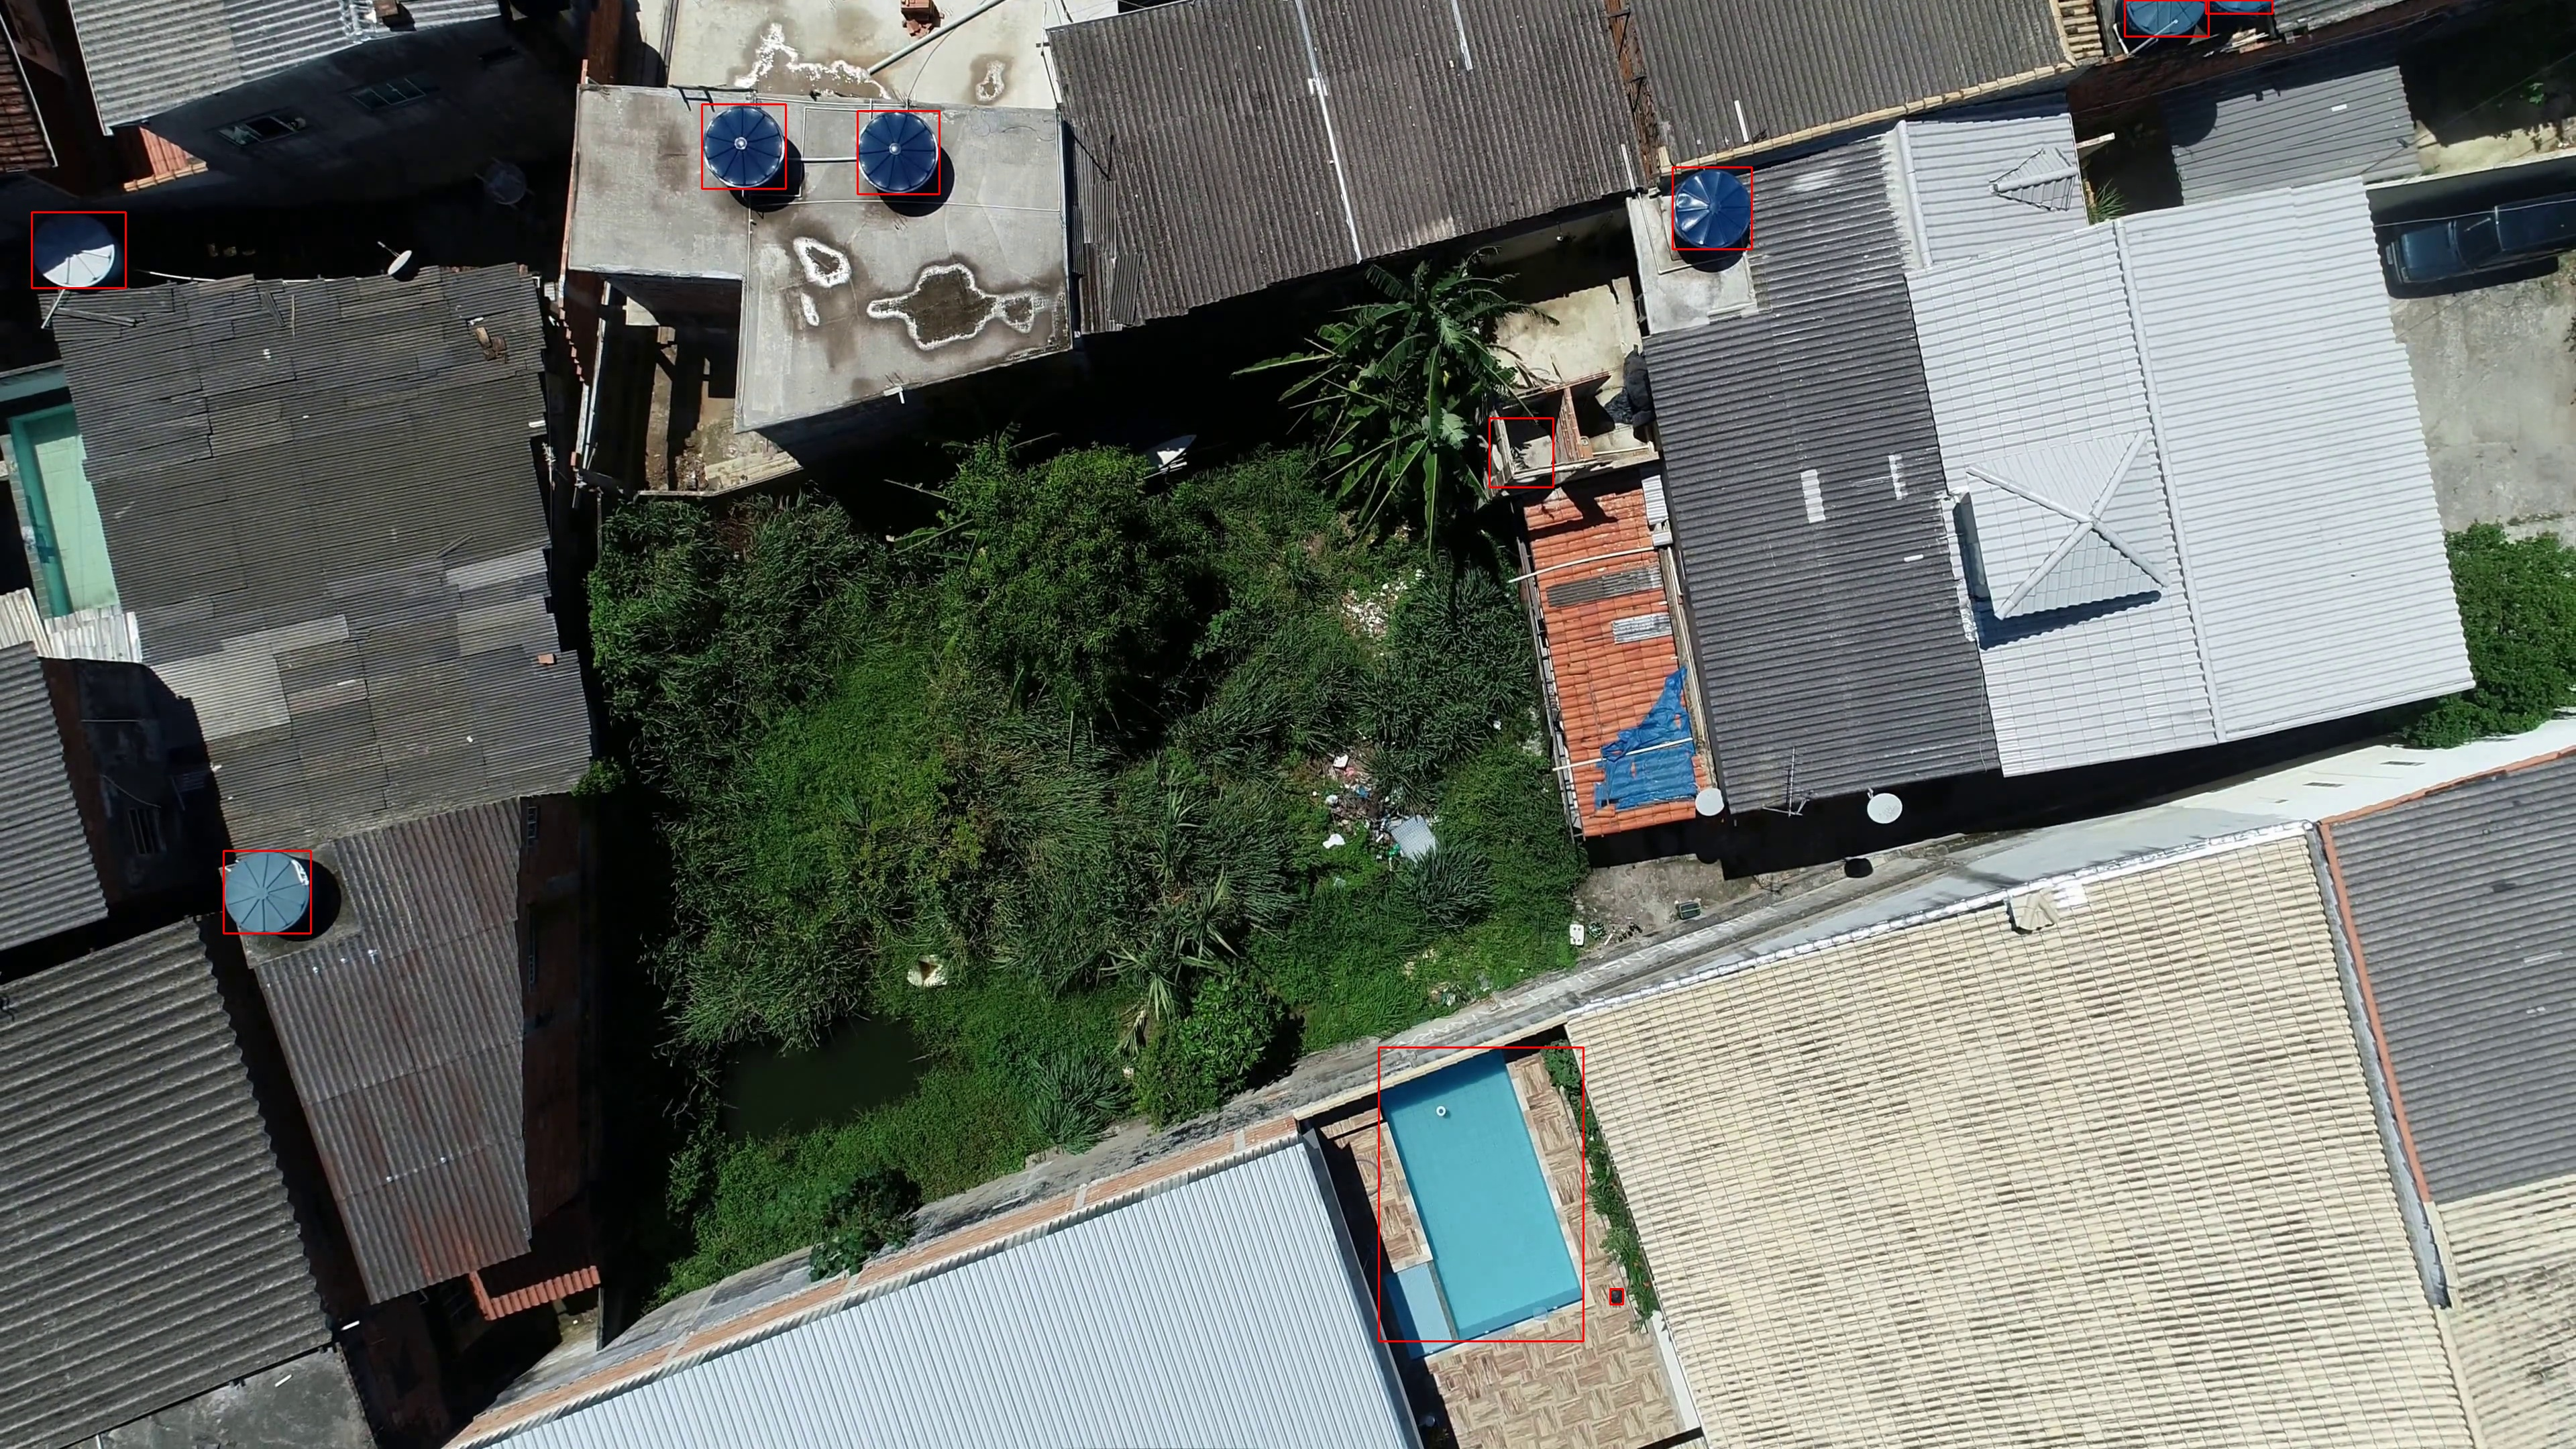
\includegraphics[width=\textwidth]{figures/introduction/uav_example_breeding_sites.jpg}
    \caption{Beispiel einer UAV-Aufnahme aus einem urbanen Gebiet mit potenziellen Brutstätten. Kleine Objekte wie Wassertanks, Reifen, Eimer oder Abflüsse sind aus der Vogelperspektive häufig schwer vom komplexen Hintergrund zu unterscheiden.}
    \label{fig:intro_uav_example}
\end{figure}

Abbildung~\ref{fig:intro_uav_example} verdeutlicht die zentrale Herausforderung dieser Arbeit. Potenzielle Brutstätten erscheinen in UAV-Aufnahmen häufig sehr klein, liegen in komplexen Dach- oder Straßenstrukturen und können visuell leicht mit Hintergrundobjekten verwechselt werden.

Ein zentrales Problem beim Training solcher Modelle ist der hohe Aufwand für manuelle Annotationen. Für überwachte Lernverfahren werden große Mengen korrekt annotierter Trainingsdaten benötigt. Bei UAV-Videos ist dieser Aufwand besonders hoch, da eine Videosequenz aus vielen Einzelbildern besteht und Objekte über zahlreiche Frames hinweg markiert werden müssten. Gleichzeitig unterscheiden sich die Erscheinungsformen potenzieller Brutstätten je nach Perspektive, Umgebung, Beleuchtung und Objektgröße. Dies erschwert nicht nur die Modellierung, sondern auch die konsistente manuelle Annotation.

Der in dieser Arbeit verwendete MBG-V2-Datensatz enthält UAV-Videodaten urbaner Gebiete sowie Annotationen potenzieller Brutstätten von \textit{Aedes aegypti}~\cite{passos2024mbgv2}. Die Daten bieten eine geeignete Grundlage, um Verfahren zur automatischen Objekterkennung und Annotation in UAV-Videos zu untersuchen. Gleichzeitig zeigen die Daten typische Herausforderungen realer Anwendungsszenarien: stark unausgewogene Klassenverteilungen, kleine Objektgrößen, komplexe Hintergründe und eine große Anzahl nicht direkt manuell annotierter Zwischenframes.

Vor diesem Hintergrund untersucht diese Arbeit einen semi-supervisierten Ansatz zur automatischen Annotation von UAV-Videodaten. Ausgangspunkt ist eine begrenzte Menge manuell annotierter Frames. Auf dieser Grundlage wird ein YOLO-basiertes Objekterkennungsmodell trainiert. Anschließend wird das trainierte Modell genutzt, um zusätzliche Annotationen auf zunächst unannotierten Frames zu erzeugen. Diese automatisch erzeugten Annotationen werden als Pseudo-Labels bezeichnet. Ergänzend wird ein Tracking-Verfahren eingesetzt, um Detektionen über mehrere aufeinanderfolgende Frames hinweg zeitlich zu verknüpfen. Dadurch soll untersucht werden, ob die zeitliche Struktur von Videodaten genutzt werden kann, um automatisch erzeugte Labels zu stabilisieren.

\subsection{Problemstellung}

Die automatische Erkennung potenzieller Brutstätten in UAV-Aufnahmen ist aus mehreren Gründen anspruchsvoll. Erstens sind viele Zielobjekte in den Luftbildern sehr klein. Dies betrifft insbesondere Objekte wie Flaschen, Plastikbeutel, kleinere Müllbehälter oder Abflüsse. Bei solchen Klassen können bereits geringe Lokalisierungsfehler dazu führen, dass die vorhergesagte Bounding Box nicht ausreichend mit der tatsächlichen Objektposition übereinstimmt.

Zweitens weisen die Daten eine starke Klassenungleichverteilung auf. Häufig vorkommende Klassen wie \textit{watertank} sind deutlich stärker vertreten als seltene Klassen wie \textit{bottle}, \textit{plastic bag} oder \textit{large trash bin}. Ein Modell kann dadurch dazu tendieren, dominante Klassen besser zu lernen, während seltene Klassen instabil oder gar nicht erkannt werden.

Drittens enthalten UAV-Videos viele visuell komplexe Hintergrundstrukturen. Dachflächen, Schatten, Wasserflächen, Straßen, technische Anlagen und runde oder rechteckige Objekte können potenziellen Brutstätten ähneln. Dadurch entstehen False Positives, bei denen Hintergrundbereiche fälschlicherweise als Objekt erkannt werden. Gleichzeitig können tatsächliche Objekte übersehen werden, wenn sie verdeckt, sehr klein oder kontrastarm sind.

Viertens ist die manuelle Annotation von Videodaten besonders zeitintensiv. Selbst wenn einzelne Frames manuell annotiert werden, bleiben zahlreiche Zwischenframes ungenutzt. Eine vollständige manuelle Annotation aller Frames ist in der Praxis häufig nicht realistisch. Daraus ergibt sich die Frage, ob ein Modell, das auf wenigen manuell annotierten Frames trainiert wurde, zur automatischen Erweiterung des Trainingsdatensatzes beitragen kann.

\subsection{Zielsetzung der Arbeit}

Ziel dieser Arbeit ist es, zu untersuchen, inwieweit ein semi-supervisierter Annotationsansatz den manuellen Annotierungsaufwand bei UAV-Videodaten reduzieren kann. Dafür wird ein YOLOv8-Modell~\cite{Ultralytics2023} zunächst auf manuell annotierten Frames trainiert. Dieses Baseline-Modell dient als Ausgangspunkt für die automatische Generierung zusätzlicher Pseudo-Labels. Anschließend wird analysiert, ob diese Pseudo-Labels die Trainingsdaten sinnvoll erweitern und welche Auswirkungen sie auf die Modellleistung haben.

Darüber hinaus wird untersucht, welche Rolle Tracking bei der Stabilisierung automatisch erzeugter Labels spielen kann. Da UAV-Daten als Videos vorliegen, enthalten sie eine zeitliche Struktur, die bei Einzelbildverfahren nicht genutzt wird. Objekte erscheinen häufig über mehrere aufeinanderfolgende Frames hinweg. Ein Tracking-Verfahren wie ByteTrack~\cite{bytetrack} kann genutzt werden, um solche Detektionen über die Zeit hinweg miteinander zu verbinden. Dadurch können stabile Objekttracks entstehen, die als zusätzliche Grundlage für eine tracking-basierte Label-Propagation dienen.

Die Arbeit verfolgt dabei nicht das Ziel, ein vollständig produktionsreifes Detektionssystem bereitzustellen. Stattdessen steht die experimentelle Untersuchung eines Annotationsworkflows im Vordergrund. Bewertet wird, ob die Kombination aus manuell annotierten Frames, Pseudo-Labeling und Tracking geeignet ist, zusätzliche Trainingsdaten zu erschließen und typische Probleme der automatischen Annotation sichtbar zu machen.

\subsection{Forschungsfragen}

Aus der beschriebenen Problemstellung ergeben sich die folgenden Forschungsfragen:

\begin{enumerate}
    \item Inwieweit kann ein YOLO-basiertes Baseline-Modell auf Grundlage einer
          begrenzten Menge manuell annotierter UAV-Frames potenzielle Brutstätten
          erkennen?

    \item Kann die automatische Pseudo-Label-Generierung den Trainingsdatensatz
          sinnvoll erweitern und die Klassenabdeckung verbessern?

    \item Welche Auswirkungen haben automatisch erzeugte Pseudo-Labels auf die
          Modellleistung, insbesondere auf Precision, Recall, mAP@50 und mAP@50--95?

    \item Inwieweit kann tracking-basierte Label-Propagation dazu beitragen,
          automatisch erzeugte Annotationen über mehrere Frames hinweg zeitlich zu
          stabilisieren und die Qualität der Pseudo-Label-Auswahl im anschließenden
          Training zu verbessern?

    \item Welche typischen Fehlerquellen treten bei der automatischen Annotation
          von UAV-Videodaten auf?
\end{enumerate}

Diese Fragen werden anhand quantitativer Modellmetriken sowie qualitativer
Beispiele untersucht. Die quantitative Auswertung umfasst Trainingskurven,
Precision-Recall-Kurven, F1-Confidence-Kurven, Konfusionsmatrizen und
mAP-Werte. Ergänzend werden die detection-basierte Pseudo-Labeling-Stufe und
die tracking-basierte Label-Propagation auf demselben manuell annotierten
Validierungssplit miteinander verglichen. Die qualitative Analyse betrachtet
beispielhafte Detektionen, Pseudo-Labels und tracking-basierte Frame-Sequenzen.

\subsection{Beitrag der Arbeit}

Der Beitrag dieser Arbeit liegt in der experimentellen Untersuchung eines
semi-supervisierten Workflows zur automatischen Annotation von UAV-Videodaten.
Im Unterschied zu rein überwachten Ansätzen wird nicht ausschließlich betrachtet,
wie gut ein Modell auf einem vollständig manuell annotierten Datensatz trainiert
werden kann. Stattdessen wird untersucht, ob ein initial trainiertes Modell genutzt
werden kann, um zusätzliche Annotationen automatisch zu erzeugen und damit den
manuellen Annotierungsaufwand zu reduzieren.

Die Arbeit leistet damit drei zentrale Beiträge. Erstens wird ein Baseline-Modell
auf manuell annotierten Frames des MBG-V2-Datensatzes trainiert und anhand
standardisierter Objekterkennungsmetriken bewertet. Zweitens wird eine
detection-basierte Pseudo-Labeling-Stufe untersucht, in der automatisch erzeugte
Labels zur Erweiterung des Trainingsdatensatzes verwendet werden. Drittens wird
die zeitliche Struktur der UAV-Videos durch ByteTrack genutzt, um
tracking-basierte Pseudo-Labels zu erzeugen. Diese werden nicht nur qualitativ
hinsichtlich ihrer zeitlichen Konsistenz betrachtet, sondern auch in einem eigenen
Retraining-Schritt quantitativ mit dem Baseline-Modell und dem
detection-basierten Pseudo-Labeling verglichen.

Ein besonderer Fokus liegt dabei auf den praktischen Grenzen des Ansatzes. Die
Arbeit zeigt nicht nur erfolgreiche Detektionen, sondern untersucht auch
Fehlerfälle wie False Positives, nicht erkannte Objekte, Klassenverwechslungen
und instabile Vorhersagen. Dadurch wird sichtbar, unter welchen Bedingungen
Pseudo-Labeling und Tracking hilfreich sind und in welchen Fällen zusätzliche
Qualitätskontrolle erforderlich bleibt.
